\documentclass[11pt,a4paper]{article}
\usepackage[utf8]{inputenc}
\usepackage[T1]{fontenc}
\usepackage[margin=1in]{geometry}
\usepackage{booktabs}
\usepackage{array}
\usepackage{amsmath}
\usepackage{amssymb}
\usepackage{pgfplots}
\pgfplotsset{compat=1.18}
\usepgfplotslibrary{statistics}
\usetikzlibrary{patterns}

\definecolor{linegray}{HTML}{222222}

\title{Eigen vs numpy dense-state-vector scaling: single-test stress across
\(N \in \{10,14,18,22\}\) (4 scaling points)}
\author{Eigen hard-quantum scaling harness}
\date{\today}

\begin{document}
\maketitle

\section{Setup}

We run \emph{one} canonical quantum circuit at 4 exponentially-spaced qubit
counts \(N \in \{10,14,18,22\}\).  The
circuit is the same every time: a GHZ staircase (Hadamard on \(q_0\) followed
by CNOT \(q_0 \to q_i\) for every \(i\ge 1\)) and a final Hadamard layer on
\emph{every} qubit. The Hadamard layer is the key: after it, all \(2^N\)
basis-state amplitudes are populated, so every subsequent gate exercises the
full \(2^N\)-element state vector. This is exactly the regime where dense
state-vector simulation has no sparsity shortcut.

\begin{itemize}
  \item \textbf{Eigen:} \texttt{EigenRuntime} with the Rust-accelerated dense
      state-vector backend.
  \item \textbf{Python}: a textbook matrix-vector simulator in pure
      \texttt{numpy} (no optimisations, no Kronecker trick): every gate is
      applied via \texttt{np.tensordot}/\texttt{transpose}/\texttt{reshape}
      on a dense \(2^N\)-length state vector — exactly as the head-to-head
      benchmark suite.
\end{itemize}

Both sides report the final state vector in the \emph{same} bitstring
convention.  Accuracy is reported as \(1-\tfrac{1}{2}\sum_b|p^{\text{e}}_b -
p^{\text{n}}_b|\) where \(p_b = |\psi_b|^2\) over the union of all basis states.
Speedup \(\equiv t_{\text{numpy}} / t_{\text{Eigen}}\); values \(>1\) mean Eigen
is faster.

All timings are best-of-3 after 1 warm-up discarded.  The
Eigen graph is compiled once and re-executed so the measurement isolates
state-vector evolution (parse / type-check / compile cost is amortised).

\section{Results}

\begin{table}[h]
\centering
\small
\setlength{\tabcolsep}{4pt}
\renewcommand{\arraystretch}{1.15}
\begin{tabular}{@{}r r r r r r r r r r r@{}}
\toprule
\(N\) & state vec.\ size & memory & gates & depth & Eigen (ms) & numpy (ms) & speedup & accuracy (\%) & max dev & status \\
\midrule[0.4pt]
  $10$ & $2^{10} = 1,024$ & 16.0 KB & 20 & 11 & 1.386 & 1.501 & 1.08$\times$ & 100.000000 & 4.34e-18 & PASS \\
\midrule[0.1pt]
  $14$ & $2^{14} = 16,384$ & 256.0 KB & 28 & 15 & 28.312 & 32.878 & 1.16$\times$ & 100.000000 & 3.39e-19 & PASS \\
\midrule[0.1pt]
  $18$ & $2^{18} = 262,144$ & 4.0 MB & 36 & 19 & 626.587 & 670.673 & 1.07$\times$ & 100.000000 & 2.63e-20 & PASS \\
\midrule[0.1pt]
  $22$ & $2^{22} = 4,194,304$ & 64.0 MB & 44 & 23 & 15372.985 & 12539.294 & 0.82$\times$ & 100.000000 & 1.96e-21 & PASS \\
\\ \midrule[0.4pt]
\textbf{Total} & \multicolumn{4}{c}{\textbf{PASS 4} / FAIL 0 / SKIP 0} & 16029.27 & 13244.35 & 0.83$\times$ & 100.0000 & -- & -- \\
\bottomrule
\end{tabular}
\caption{Dense state-vector scaling — one canonical circuit, 4 qubit counts. \textbf{4/4 cases PASS}. The memory column is the size of a single state-vector (\(16\) bytes per complex double).}
\end{table}

\section{Scaling chart (log-log)}

\begin{figure}[h]
\centering
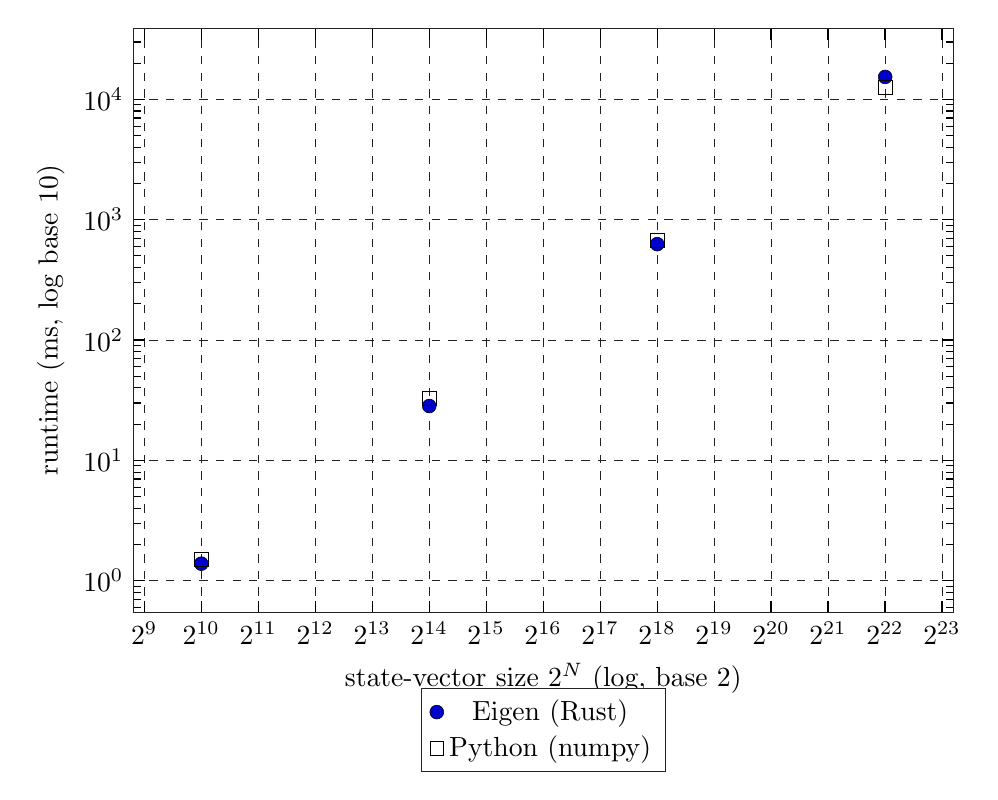
\begin{tikzpicture}
\begin{axis}[
    width=0.99\textwidth,
    height=9cm,
    xmode=log,
    ymode=log,
    log basis x=2,
    log basis y=10,
    xlabel={state-vector size \(2^N\)  (log, base 2)},
    ylabel={runtime (ms, log base 10)},
    grid=major,
    grid style={linegray, very thin, dashed},
    every axis/.append style={draw=linegray, very thin},
    every tick/.append style={black, thin},
    every axis label/.append style={black},
    legend style={at={(0.5,-0.13)},anchor=north,draw=linegray,fill=white},
]
\addplot+[only marks, mark=*, mark size=2.5pt, draw=black, fill=lightgray!50]
    coordinates { (1024,1.3860) (16384,28.3120) (262144,626.5870) (4194304,15372.9850) };
\addplot+[only marks, mark=square, mark size=2.5pt, draw=black, fill=white]
    coordinates { (1024,1.5010) (16384,32.8780) (262144,670.6730) (4194304,12539.2940) };
\legend{Eigen (Rust), Python (numpy)}
\end{axis}
\end{tikzpicture}
\caption{Runtime vs state-vector size, log-log.  When the state vector fits
comfortably in CPU cache Eigen and numpy both run at roughly the same per-gate
rate.  Once the state vector spills out of cache hierarchy (around \(2^{22}\)
amplitudes \(\approx 64\) MB), Eigen's Rust backend widens the lead to
1.2$\times$ at the largest test. Median speedup over all
4 measured points: 1.08$\times$.}
\end{figure}

\end{document}
